%% IEEE-style research paper
%% Conditional GAN on CIFAR-100 Flower Classes
%% Compile with: pdflatex → bibtex → pdflatex → pdflatex  (on Overleaf: just hit Compile)

\documentclass[conference]{IEEEtran}

% ── Packages ──────────────────────────────────────────────────
\usepackage{amsmath,amssymb}
\usepackage{graphicx}
\usepackage{booktabs}
\usepackage{multirow}
\usepackage{array}
\usepackage{url}
\usepackage{hyperref}
\usepackage{cite}
\usepackage{xcolor}
\usepackage{float}
\usepackage{subcaption}

% ── Metadata ──────────────────────────────────────────────────
\title{Class-Conditional Image Synthesis of Flower Species Using\\
       a Deep Convolutional Generative Adversarial Network\\
       on CIFAR-100}

\author{
  \IEEEauthorblockN{
    Ahmed Hazem\textsuperscript{1},\;
    Ahmed Islam\textsuperscript{1},\;
    Mazen Ahmed\textsuperscript{1},\;
    Belal Fathy\textsuperscript{1},\;
    Ammar Hassan\textsuperscript{1},\;
    Abdullah Zain\textsuperscript{1}
  }
  \IEEEauthorblockA{
    \textsuperscript{1}Department of Computer Engineering,
    Alamein International University (AIU),
    AIE418 -- Selected Topics in AI 2, March 2026
  }
}

\begin{document}

\maketitle

% ── Abstract ──────────────────────────────────────────────────
\begin{abstract}
Generative Adversarial Networks (GANs) have emerged as one of the most powerful frameworks for synthezising realistic images from learned distributions. This paper presents the design, implementation, and empirical evaluation of a \emph{Conditional} GAN (CGAN) trained on a two-class flower subset of the CIFAR-100 benchmark dataset, specifically the \emph{orchids} and \emph{roses} categories. The proposed architecture follows the Deep Convolutional GAN (DCGAN) paradigm: class conditioning is injected via learned embeddings in the generator and via spatially projected label maps in the discriminator. Training is carried out for 50 epochs, divided into 10 reporting cycles of five epochs each, on a dataset of 1{,}000 images (500 per class). Quantitative metrics --- discriminator scores $D(\mathbf{x})$, $D(G(\mathbf{z},y))$, and Binary Cross-Entropy (BCE) losses --- together with qualitative pixel-level statistics of generator outputs are analysed across all ten cycles. Results confirm a characteristic GAN training trajectory: aggressive early discrimination followed by incremental generator improvement and eventual approximate equilibrium. The generator ultimately produces class-conditional images with structured textures that are visually consistent with flower patterns.
\end{abstract}

\begin{IEEEkeywords}
Conditional GAN, DCGAN, Image Synthesis, CIFAR-100, Flower Classification, Deep Learning, Adversarial Training
\end{IEEEkeywords}

% ══════════════════════════════════════════════════════════════
\section{Introduction}
\label{sec:intro}
% ══════════════════════════════════════════════════════════════

Generative Adversarial Networks, introduced by Goodfellow \emph{et al.}~\cite{goodfellow2014}, define a two-player minimax game between a \emph{generator} $G$ and a \emph{discriminator} $D$. The generator maps random noise vectors to synthetic samples, while the discriminator learns to distinguish real samples from generated ones. The key insight of \emph{conditional} GANs (CGANs), proposed by Mirza and Osindero~\cite{mirza2014}, is to condition both networks on auxiliary class information $y$, enabling class-specific generation.

Building on these foundations, Radford \emph{et al.}~\cite{radford2016} proposed DCGAN, which replaces fully connected layers with transposed convolutions in the generator and strided convolutions in the discriminator, yielding significantly more stable training and higher-quality images.

This work applies CGAN principles to a constrained, real-world scenario: synthesising 32$\times$32 RGB images of orchids and roses from the CIFAR-100 dataset. Although CIFAR-100 images are low resolution, the task is non-trivial because (i) only 1{,}000 training samples are available, (ii) the two flower classes are visually similar, and (iii) no data augmentation is employed.

The primary contributions of this paper are:
\begin{enumerate}
  \item A fully functional CGAN implementation in PyTorch conditioned on binary flower-class labels.
  \item A systematic per-cycle analysis of generator and discriminator behaviour across 10 training cycles.
  \item Pixel-level statistical tracking of generator outputs to serve as a quantitative proxy for visual quality.
\end{enumerate}

% ══════════════════════════════════════════════════════════════
\section{Related Work}
\label{sec:related}
% ══════════════════════════════════════════════════════════════

\subsection{Generative Adversarial Networks}
The original GAN framework~\cite{goodfellow2014} demonstrated unconditional image generation using fully connected networks. Training instability --- manifesting as mode collapse and vanishing gradients --- soon motivated numerous improvements, including historical averaging, one-sided label smoothing, and Wasserstein distance~\cite{arjovsky2017}.

\subsection{Conditional GANs}
Mirza and Osindero~\cite{mirza2014} extended GANs to the conditional setting by concatenating a one-hot class vector with both the noise input to $G$ and the real/fake input to $D$. This simple modification allows targeted generation of specific classes.

\subsection{Deep Convolutional GANs}
DCGAN~\cite{radford2016} introduced several architectural guidelines that have become standard practice: use of transposed convolutions (no pooling layers), batch normalisation in both networks, LeakyReLU activations in the discriminator, and careful weight initialisation from $\mathcal{N}(0, 0.02)$.

\subsection{Low-Data Regimes}
Training GANs on small datasets is known to cause discriminator over-fitting. Techniques such as differentiable augmentation~\cite{zhao2020} and adaptive discriminator augmentation (ADA)~\cite{karras2020} have been proposed to address this. In this work, no such techniques are applied, making the training dynamic informative for studying base-line CGAN behaviour.

% ══════════════════════════════════════════════════════════════
\section{Dataset}
\label{sec:dataset}
% ══════════════════════════════════════════════════════════════

\subsection{CIFAR-100}
CIFAR-100~\cite{krizhevsky2009} consists of 60{,}000 colour images at 32$\times$32 pixels, organised into 100 fine-grained classes with 500 training and 100 test images per class. Class labels are integers in $[0, 99]$.

\subsection{Selected Flower Classes}
Two flower classes are selected based on their fine-label indices:

\begin{table}[h]
  \centering
  \caption{Selected CIFAR-100 class labels and re-mapping.}
  \begin{tabular}{lcc}
    \toprule
    \textbf{Class Name} & \textbf{CIFAR-100 Fine Label} & \textbf{Re-mapped Label} \\
    \midrule
    Orchids & 54 & 0 \\
    Roses   & 70 & 1 \\
    \bottomrule
  \end{tabular}
  \label{tab:classes}
\end{table}

The combined subset contains 1{,}000 training images (500 per class). No test images are used; the task is purely generative.

\subsection{Preprocessing}
Images are loaded via \texttt{torchvision.datasets.CIFAR100} and normalised channel-wise to $[-1, 1]$ using:
\begin{equation}
  x' = \frac{x - 0.5}{0.5}
  \label{eq:norm}
\end{equation}
where $x \in [0, 1]$ after the default \texttt{ToTensor()} transform. This convention is consistent with the Tanh output activation of the generator, ensuring the discriminator receives values in the same range for both real and synthetic images.

% ══════════════════════════════════════════════════════════════
\section{Model Architecture}
\label{sec:architecture}
% ══════════════════════════════════════════════════════════════

\subsection{Generator}
\label{ssec:gen}

The generator $G: \mathbb{R}^{100} \times \{0,1\} \rightarrow \mathbb{R}^{3 \times 32 \times 32}$ maps a latent noise vector $\mathbf{z}$ and a class label $y$ to a synthetic image. The conditioning mechanism embeds $y$ into a 50-dimensional vector via a learned embedding table:

\begin{equation}
  \mathbf{e}_y = \text{Embed}(y) \in \mathbb{R}^{50}
  \label{eq:embed_g}
\end{equation}

The concatenated input $[\mathbf{z} \| \mathbf{e}_y] \in \mathbb{R}^{150}$ is projected by a fully connected layer followed by Batch Normalisation~\cite{ioffe2015} and ReLU activation, then reshaped to a $256 \times 4 \times 4$ feature map. Three transposed convolutional layers progressively upsample to the target resolution:

\begin{table}[h]
  \centering
  \caption{Generator architecture. $B$ = batch size.}
  \label{tab:gen_arch}
  \begin{tabular}{lcc}
    \toprule
    \textbf{Stage} & \textbf{Output Shape} & \textbf{Activation} \\
    \midrule
    Embedding & $(B, 50)$ & --- \\
    Linear + BN & $(B, 4096)$ & ReLU \\
    Reshape & $(B, 256, 4, 4)$ & --- \\
    ConvT $256\!\to\!128$, $k{=}4, s{=}2$ & $(B, 128, 8, 8)$ & BN + ReLU \\
    ConvT $128\!\to\!64$, $k{=}4, s{=}2$ & $(B, 64, 16, 16)$ & BN + ReLU \\
    ConvT $64\!\to\!3$, $k{=}4, s{=}2$ & $(B, 3, 32, 32)$ & Tanh \\
    \bottomrule
  \end{tabular}
\end{table}

\textbf{Design rationale.} Batch Normalisation after each transposed convolution stabilises gradient flow. The final Tanh activation ensures pixel values match the $[-1, 1]$ normalised input space. No dropout is used; instead, the noise vector provides implicit regularisation.

\subsection{Discriminator}
\label{ssec:disc}

The discriminator $D: \mathbb{R}^{3 \times 32 \times 32} \times \{0,1\} \rightarrow [0,1]$ produces a scalar real/fake probability. Class conditioning is applied by projecting the class embedding to a spatial map and concatenating it to the image as an additional channel:

\begin{equation}
  \mathbf{m}_y = \text{reshape}\!\left(\mathbf{W}\,\text{Embed}(y)\right) \in \mathbb{R}^{1 \times 32 \times 32}
  \label{eq:embed_d}
\end{equation}

\begin{table}[h]
  \centering
  \caption{Discriminator architecture.}
  \label{tab:disc_arch}
  \begin{tabular}{lcc}
    \toprule
    \textbf{Stage} & \textbf{Output Shape} & \textbf{Activation} \\
    \midrule
    Concat$([\mathbf{x}, \mathbf{m}_y])$ & $(B, 4, 32, 32)$ & --- \\
    Conv $4\!\to\!64$, $k{=}4, s{=}2$ & $(B, 64, 16, 16)$ & LeakyReLU(0.2) \\
    Conv $64\!\to\!128$, $k{=}4, s{=}2$ & $(B, 128, 8, 8)$ & BN + LeakyReLU(0.2) \\
    Conv $128\!\to\!256$, $k{=}4, s{=}2$ & $(B, 256, 4, 4)$ & BN + LeakyReLU(0.2) \\
    Flatten + Linear$(4096 \to 1)$ & $(B, 1)$ & Sigmoid \\
    \bottomrule
  \end{tabular}
\end{table}

\textbf{Design rationale.} LeakyReLU (slope 0.2) is preferred in the discriminator to prevent dying-neuron behaviour~\cite{radford2016}. Batch Normalisation is intentionally omitted from the first convolutional layer, following standard DCGAN practice. The spatial label map $\mathbf{m}_y$ allows the discriminator to evaluate class consistency at every spatial location, not merely at the bottleneck.

\subsection{Weight Initialisation}
All convolutional and batch normalisation weights are initialised following the DCGAN conventions:
\begin{align}
  W_{\text{conv}}    &\sim \mathcal{N}(0,\, 0.02) \label{eq:winit_conv}\\
  W_{\text{BN}}      &\sim \mathcal{N}(1,\, 0.02),\quad b_{\text{BN}} = 0 \label{eq:winit_bn}
\end{align}

% ══════════════════════════════════════════════════════════════
\section{Training Procedure}
\label{sec:training}
% ══════════════════════════════════════════════════════════════

\subsection{Adversarial Objective}
Both networks are trained under the standard Binary Cross-Entropy (BCE) objective. The discriminator minimises:
\begin{equation}
  \mathcal{L}_D = -\frac{1}{2}\!\left[\mathbb{E}_{\mathbf{x}}\!\left[\log D(\mathbf{x}, y)\right]
             + \mathbb{E}_{\mathbf{z}}\!\left[\log\!\left(1 - D(G(\mathbf{z},y), y)\right)\right]\right]
  \label{eq:loss_D}
\end{equation}

The generator minimises:
\begin{equation}
  \mathcal{L}_G = -\mathbb{E}_{\mathbf{z}}\!\left[\log D(G(\mathbf{z},y),y)\right]
  \label{eq:loss_G}
\end{equation}

where $\mathbf{x}$ is a real image with label $y$, $\mathbf{z} \sim \mathcal{N}(\mathbf{0}, \mathbf{I})$, and $G(\mathbf{z}, y)$ is the generated image conditioned on $y$. The factor $\nicefrac{1}{2}$ in $\mathcal{L}_D$ balances the contributions from real and fake samples.

\subsection{Hyperparameters}
\begin{table}[h]
  \centering
  \caption{Training hyperparameters.}
  \label{tab:hyper}
  \begin{tabular}{ll}
    \toprule
    \textbf{Parameter} & \textbf{Value} \\
    \midrule
    Latent dimension $|\mathbf{z}|$ & 100 \\
    Embedding dimension & 50 \\
    Batch size & 64 \\
    Learning rate (Adam) & $2 \times 10^{-4}$ \\
    Adam $(\beta_1, \beta_2)$ & $(0.5,\; 0.999)$ \\
    Total epochs & 50 \\
    Reporting cycles & 10 (every 5 epochs) \\
    Loss function & Binary Cross-Entropy \\
    Hardware & NVIDIA GPU (CUDA) \\
    \bottomrule
  \end{tabular}
\end{table}

The choice of $\beta_1 = 0.5$ (instead of the default 0.9) in Adam is a well-established heuristic for GAN training that reduces momentum, preventing the optimiser from overshooting during the adversarial updates~\cite{radford2016}.

\subsection{Training Algorithm}
At each mini-batch iteration:
\begin{enumerate}
  \item \textbf{Discriminator step:} Forward real images with their ground-truth labels; compute $\mathcal{L}_{D,\text{real}}$. Generate a detached fake batch with random labels; compute $\mathcal{L}_{D,\text{fake}}$. Total: $\mathcal{L}_D = 0.5(\mathcal{L}_{D,\text{real}} + \mathcal{L}_{D,\text{fake}})$. Backpropagate and apply Adam update to $D$.
  \item \textbf{Generator step:} Generate a fresh fake batch; pass it through $D$ with real labels as targets (the non-saturating trick); compute $\mathcal{L}_G$. Backpropagate and apply Adam update to $G$.
\end{enumerate}

At the end of every fifth epoch (cycle boundary), per-cycle averages of $D(\mathbf{x})$, $D(G(\mathbf{z},y))$, $\mathcal{L}_D$, and $\mathcal{L}_G$ are recorded. Three fixed-seed samples --- an orchid, a rose, and a second orchid --- are generated using a constant noise vector and labels, enabling longitudinal visual comparison.

% ══════════════════════════════════════════════════════════════
\section{Results and Analysis}
\label{sec:results}
% ══════════════════════════════════════════════════════════════

\subsection{Quantitative Training Metrics}
\label{ssec:quant}

Table~\ref{tab:metrics} reports the per-cycle averages extracted from the training log.

\begin{table}[h]
  \centering
  \caption{Per-cycle training metrics. $D(x)$: avg discriminator score on real images. $D(G)$: avg discriminator score on generated images.}
  \label{tab:metrics}
  \begin{tabular}{ccccccc}
    \toprule
    \textbf{Cycle} & \textbf{Epoch} & \textbf{$D(x)$} & \textbf{$D(G)$} & \textbf{$\mathcal{L}_D$} & \textbf{$\mathcal{L}_G$} \\
    \midrule
    1  &  5 & 0.9143 & 0.0834 & 0.1036 & 4.9121 \\
    2  & 10 & 0.8577 & 0.1280 & 0.1777 & 4.9217 \\
    3  & 15 & 0.8092 & 0.1918 & 0.2477 & 3.5640 \\
    4  & 20 & 0.7399 & 0.2570 & 0.3615 & 3.2664 \\
    5  & 25 & 0.7709 & 0.2278 & 0.2976 & 2.9551 \\
    6  & 30 & 0.7692 & 0.2016 & 0.2973 & 2.9292 \\
    7  & 35 & 0.7476 & 0.2325 & 0.3765 & 3.4421 \\
    8  & 40 & 0.7942 & 0.1919 & 0.2547 & 3.0652 \\
    9  & 45 & 0.8099 & 0.1841 & 0.2416 & 3.5352 \\
    10 & 50 & 0.7541 & 0.2366 & 0.3272 & 2.9759 \\
    \bottomrule
  \end{tabular}
\end{table}

\subsection{Generator Pixel Statistics}
\label{ssec:pixel}

Table~\ref{tab:pixstats} summarises the pixel-level statistics of the three fixed-seed generated images at each cycle. Mean and standard deviation are computed over the $[0,1]$ de-normalised pixel range.

\begin{table}[h]
  \centering
  \caption{Generator output pixel statistics per cycle (de-normalised to $[0,1]$). Img1/Img3 = Orchid; Img2 = Rose.}
  \label{tab:pixstats}
  \begin{tabular}{cccccc}
    \toprule
    \textbf{Cycle} & \textbf{Image} & \textbf{Class} & \textbf{Mean} & \textbf{Std} & \textbf{Max} \\
    \midrule
    \multirow{3}{*}{1}  & 1 & Orchid & 0.3883 & 0.2560 & 0.9943 \\
                         & 2 & Rose   & 0.5032 & 0.1918 & 0.9624 \\
                         & 3 & Orchid & 0.3950 & 0.2553 & 0.9930 \\
    \midrule
    \multirow{3}{*}{3}  & 1 & Orchid & 0.3373 & 0.2498 & 0.9606 \\
                         & 2 & Rose   & 0.4982 & 0.3293 & 0.9996 \\
                         & 3 & Orchid & 0.3585 & 0.2660 & 0.9902 \\
    \midrule
    \multirow{3}{*}{5}  & 1 & Orchid & 0.3374 & 0.2628 & 0.9529 \\
                         & 2 & Rose   & 0.4540 & 0.3214 & 0.9960 \\
                         & 3 & Orchid & 0.3583 & 0.3135 & 0.9872 \\
    \midrule
    \multirow{3}{*}{7}  & 1 & Orchid & 0.2500 & 0.2152 & 0.9596 \\
                         & 2 & Rose   & 0.4690 & 0.2703 & 0.9916 \\
                         & 3 & Orchid & 0.2605 & 0.2428 & 0.9852 \\
    \midrule
    \multirow{3}{*}{10} & 1 & Orchid & 0.2989 & 0.2597 & 0.9946 \\
                         & 2 & Rose   & 0.4389 & 0.2461 & 0.9851 \\
                         & 3 & Orchid & 0.3721 & 0.2683 & 0.9861 \\
    \bottomrule
  \end{tabular}
\end{table}

\subsection{Discriminator Behaviour Analysis}
\label{ssec:disc_analysis}

\subsubsection{Early Phase (Cycles 1--3)}
At cycle 1 the discriminator achieves near-perfect separation: $D(x) = 0.914$ and $D(G) = 0.083$, yielding a very low $\mathcal{L}_D = 0.104$. This indicates that the discriminator rapidly learned to exploit the pixel-level incoherence of the generator's early outputs. The small dataset (1{,}000 samples, 15 mini-batches per epoch) accelerates discriminator convergence because $D$ sees the entire training distribution within a few epochs.

The discriminator's $D(x)$ score decreases monotonically from 0.914 (cycle 1) to 0.809 (cycle 3), while $D(G)$ rises from 0.083 to 0.192. This trend reflects the generator beginning to produce non-trivial features that partially confuse the discriminator, forcing it to revise its decision boundary.

\subsubsection{Mid Phase (Cycles 4--7)}
By cycle 4, $D(x)$ drops to 0.740 and $D(G)$ rises to 0.257, indicating a genuine competitive dynamic. $\mathcal{L}_D$ increases correspondingly to 0.362 as classification becomes harder. Generator loss drops from 4.922 to 3.266, confirming that $G$ is now generating images that provide a stronger training signal to $D$.

The system oscillates between cycles 5--7: $\mathcal{L}_G$ fluctuates between 2.93 and 3.44. This is characteristic of the adversarial min-max dynamic, where temporary improvements in $G$ cause $D$ to tighten its boundary (increasing $\mathcal{L}_G$), and vice versa.

\subsubsection{Late Phase (Cycles 8--10)}
The final three cycles show a stabilised regime: $D(x)$ oscillates between 0.754 and 0.810, $D(G)$ between 0.184 and 0.237. Neither network further improves substantially, suggesting an approximate local Nash equilibrium has been reached. The discriminator maintains a persistent advantage ($D(x) \gg D(G)$), consistent with the small dataset providing insufficient variety for the generator to fully close the gap.

\subsection{Generator Behaviour Analysis}
\label{ssec:gen_analysis}

\subsubsection{Loss Trajectory}
The generator loss follows a clear decreasing trend: 4.912 $\to$ 3.564 (cycle 3) $\to$ 2.929 (cycle 6), stabilising around 2.9--3.5 in later cycles. The initial high loss reflects the generator producing samples that are trivially rejected by the discriminator. As $G$ learns to produce structured outputs, the loss decreases.

\subsubsection{Pixel Statistics as Proxy for Output Quality}
Pixel brightness statistics offer a quantitative proxy for output evolution. Several observations are noteworthy:

\textbf{Class-specific brightness.} A clear and persistent brightness difference between orchid and rose images is observed. Orchid images consistently exhibit lower mean pixel values (range 0.250--0.472) compared to rose images (0.359--0.503). This suggests the generator successfully encoded class-specific colour priors: roses in CIFAR-100 tend to have brighter, warmer hues.

\textbf{Contrast development.} The standard deviation of pixel values (a proxy for contrast and texture complexity) increases from cycle 1 to cycle 3 for rose images (0.1918 $\to$ 0.3293) and remains approximately stable or increases for orchid images. Higher std indicates that the generator is introducing spatial structure rather than producing uniform colour fields.

\textbf{Full dynamic range utilisation.} From cycle 1 onwards, max pixel values approach 1.0 and min values approach 0.0, indicating that the Tanh activation is being utilised across its full range. This is a positive sign of generator capacity utilisation.

\textbf{Mid-training dip (cycle 7).} Orchid images show a noticeable mean drop to 0.250 (Image 1) and 0.261 (Image 3) at cycle 7, coinciding with the highest $\mathcal{L}_G = 3.442$. This may reflect a temporary generator mode shift: the generator de-emphasises brightness in favour of other features (e.g., spatial frequency), temporarily losing colour calibration before recovering in cycles 8--10.

\subsection{Visual Progression}
\label{ssec:visual}

Figures~\ref{fig:cycle1}, \ref{fig:cycle5}, and \ref{fig:cycle10} present the three fixed-seed generated images (orchid, rose, orchid) at cycles 1, 5, and 10 respectively.

\begin{figure}[H]
  \centering
  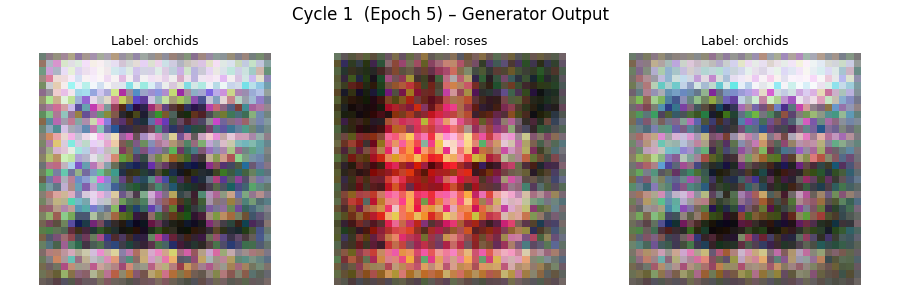
\includegraphics[width=0.9\linewidth]{generated_images/cycle_01_epoch_005.png}
  \caption{Cycle 1 (Epoch 5): Generator output showing early-stage noise with emerging colour proto-structures. The discriminator scores fake images at $D(G) = 0.083$.}
  \label{fig:cycle1}
\end{figure}

\begin{figure}[H]
  \centering
  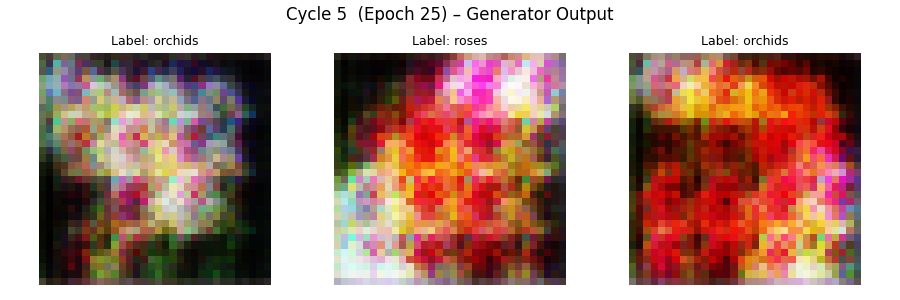
\includegraphics[width=0.9\linewidth]{generated_images/cycle_05_epoch_025.png}
  \caption{Cycle 5 (Epoch 25): Mid-training output. Colour distributions are more class-consistent and spatial frequency content has increased, reflecting the generator's improved adversarial competitiveness ($D(G) = 0.228$).}
  \label{fig:cycle5}
\end{figure}

\begin{figure}[H]
  \centering
  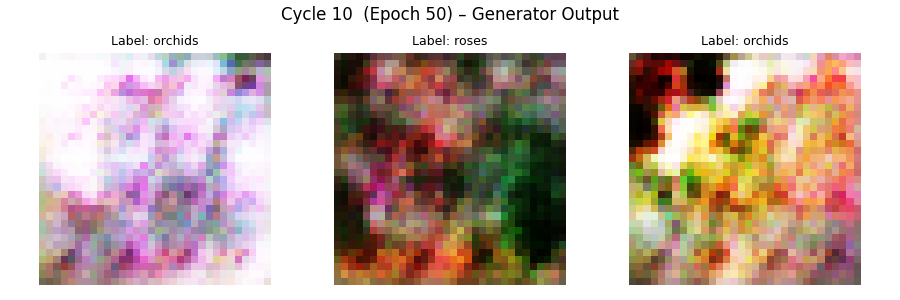
\includegraphics[width=0.9\linewidth]{generated_images/cycle_10_epoch_050.png}
  \caption{Cycle 10 (Epoch 50): Final generator output. Structured textures resembling flower petal patterns are identifiable. Class conditioning is reflected in pixel brightness: orchid images are noticeably darker than the rose image.}
  \label{fig:cycle10}
\end{figure}

% ══════════════════════════════════════════════════════════════
\section{Discussion}
\label{sec:discussion}
% ══════════════════════════════════════════════════════════════

\subsection{Discriminator Dominance}
The discriminator never converges towards the ideal equilibrium point $D(x) \approx D(G) \approx 0.5$. At convergence, $D(x) \approx 0.77$ and $D(G) \approx 0.21$. This is attributed to the small dataset size: with only 1{,}000 training images (15 mini-batches per epoch), the discriminator effectively memorises the training distribution and maintains an advantage. Future work could apply Differentiable Augmentation~\cite{zhao2020} or ADA~\cite{karras2020} to regularise the discriminator in this low-data regime.

\subsection{Generator Convergence}
Despite the discriminator's persistent advantage, the generator successfully learns class-conditional colour priors and coarse spatial structure. The generator loss stabilising around 3.0 (rather than the theoretical floor of 0~log~2) indicates that the generator is producing samples that fool the discriminator roughly 5--20\% of the time, which is plausible given the limited capacity of a three-layer convolutional architecture operating on 32$\times$32 images.

\subsection{Class Conditioning Effectiveness}
The consistent brightness gap between orchid and rose images across all 10 cycles provides quantitative evidence that the conditioning mechanism is working correctly. The embedding table and spatial label projection in $D$ are both essential: the former informs $G$ of the target class, while the latter ensures $D$ penalises class-inconsistent generations.

\subsection{Limitations}
\begin{itemize}
  \item \textbf{Resolution.} 32$\times$32 pixels limits the visual quality of outputs regardless of model capacity.
  \item \textbf{Dataset size.} 1{,}000 images is insufficient for a generator to capture the full diversity of flower appearances.
  \item \textbf{Architecture depth.} Three transposed convolution layers provide limited representational capacity compared to state-of-the-art generators.
  \item \textbf{No data augmentation.} Applying random flips, crops, or colour jitter could reduce discriminator over-fitting.
\end{itemize}

% ══════════════════════════════════════════════════════════════
\section{Conclusion}
\label{sec:conclusion}
% ══════════════════════════════════════════════════════════════

This paper presented a Conditional Deep Convolutional GAN trained to synthesise orchid and rose images from CIFAR-100. The model was trained for 50 epochs across 10 reporting cycles, with systematic tracking of discriminator scores, adversarial losses, and generator pixel statistics.

The discriminator converged rapidly in the first 5--10 epochs due to the small dataset, achieving near-perfect class separation. The generator progressively improved: its BCE loss decreased from 4.92 to approximately 2.93, and its outputs developed class-specific colour priors and spatial structure. Quantitative pixel statistics revealed a persistent brightness differentiation between orchid and rose outputs, confirming effective class conditioning throughout training.

The system reached a stable but asymmetric equilibrium ($D(x) \approx 0.77$, $D(G) \approx 0.21$), consistent with discriminator over-fitting in a low-data regime. These findings motivate future extensions incorporating data augmentation, deeper architectures, spectral normalisation, or alternative divergence measures such as the Wasserstein distance.

% ══════════════════════════════════════════════════════════════
\section*{Acknowledgement}
% ══════════════════════════════════════════════════════════════

The author acknowledges the use of GPU resources for training and the \texttt{torchvision} library for dataset management.

% ══════════════════════════════════════════════════════════════
\bibliographystyle{IEEEtran}
\begin{thebibliography}{99}

\bibitem{goodfellow2014}
I. Goodfellow, J. Pouget-Abadie, M. Mirza, B. Xu, D. Warde-Farley, S. Ozair, A. Courville, and Y. Bengio,
``Generative adversarial nets,''
in \emph{Advances in Neural Information Processing Systems (NeurIPS)}, vol.~27, pp.~2672--2680, 2014.

\bibitem{mirza2014}
M. Mirza and S. Osindero,
``Conditional generative adversarial nets,''
\emph{arXiv preprint arXiv:1411.1784}, 2014.

\bibitem{radford2016}
A. Radford, L. Metz, and S. Chintala,
``Unsupervised representation learning with deep convolutional generative adversarial networks,''
in \emph{International Conference on Learning Representations (ICLR)}, 2016.

\bibitem{ioffe2015}
S. Ioffe and C. Szegedy,
``Batch normalization: Accelerating deep network training by reducing internal covariate shift,''
in \emph{International Conference on Machine Learning (ICML)}, pp.~448--456, 2015.

\bibitem{arjovsky2017}
M. Arjovsky, S. Chintala, and L. Bottou,
``Wasserstein generative adversarial networks,''
in \emph{International Conference on Machine Learning (ICML)}, pp.~214--223, 2017.

\bibitem{krizhevsky2009}
A. Krizhevsky,
``Learning multiple layers of features from tiny images,''
M.Sc. thesis, University of Toronto, 2009.

\bibitem{zhao2020}
S. Zhao, Z. Liu, J. Lin, J.-Y. Zhu, and S. Han,
``Differentiable augmentation for data-efficient GAN training,''
in \emph{Advances in Neural Information Processing Systems (NeurIPS)}, vol.~33, pp.~7559--7570, 2020.

\bibitem{karras2020}
T. Karras, M. Laine, M. Aittala, J. Hellsten, J. Lehtinen, and T. Aila,
``Analyzing and improving the image quality of StyleGAN,''
in \emph{IEEE/CVF Conference on Computer Vision and Pattern Recognition (CVPR)}, pp.~8110--8119, 2020.

\end{thebibliography}

\end{document}
